\documentclass[12pt,preprint]{aastex}
\usepackage{savesym}
\savesymbol{singlespace}
\savesymbol{doublespace}
\usepackage{setspace}
\usepackage{amssymb,amsmath}
\usepackage{sidecap}
\usepackage{minted}
\setlength{\emergencystretch}{2em}%No overflowing references
\newcommand{\ie}{i.e.}
\newcommand{\etal}{et al.}
\newcommand{\dd}{\mathrm{d}}
\newcommand{\eg}{e.g.}
\newcommand{\eqnname}{equation}
\newcommand{\figurenames}{\figurename s}
\newcommand{\sectionname}{$\mathsection$}

\begin{document}

\title{APOGEE-2 Ancillary Proposal: The Far Disk in APOGEE-2 using Low-extinction Windows}
\author{P.I.: Jo~Bovy (IAS $\rightarrow$ Toronto);\\
  Institute for Advanced Study, Einstein Drive, Princeton, NJ 08540, USA;\\
  609-734-8369}
\email{bovy@ias.edu}

\section{Co.I.s:}
\begin{itemize}
  \itemsep-.25em
  \begin{spacing}{0.1}
  \item Brett Andrews (PITT PACC, Department of Physics and Astronomy,
University of Pittsburgh, 3941 O’Hara Street, Pittsburgh, PA 15260, USA)
  \item Jonathan C. Bird (Physics and Astronomy Department, Vanderbilt University, 1807 Station B, Nashville, TN 37235, USA)
  \item Diane Feuillet (New Mexico State University, Las Cruces, NM 88003, USA)
  \item $^\dagger$Douglas P.~Finkbeiner (Harvard-Smithsonian Center for Astrophysics, 60 Garden Street, Cambridge, MA 02138, USA)
  \item $^\dagger$Gregory Green (Harvard-Smithsonian Center for Astrophysics, 60 Garden Street, Cambridge, MA 02138, USA)
  \item Jon Holtzman (New Mexico State University, Las Cruces, NM 88003, USA)
  \item Chao Liu (Key Laboratory of Optical Astronomy, National Astronomical
Observatories, Chinese Academy of Sciences, Datun Road 20A, Beijing 100012, China)
  \item Melissa Ness  (Max-Planck-Institut f\"ur Astronomie, K\"onigstuhl 17, D-69117 Heidelberg, Germany)
  \item David L. Nidever (Department of Astronomy, University of Michigan, Ann Arbor, MI 48109, USA)
  \item Hans-Walter Rix (Max-Planck-Institut f\"ur Astronomie, K\"onigstuhl 17, D-69117 Heidelberg, Germany)
  \item Mathias Schultheis (Laboratoire Lagrange (UMR7293), Universit\'{e} de Nice Sophia Antipolis, CNRS, Observatoire de la C\^{o}te d'Azur, BP 4229, 06304 Nice Cedex 4, France)
\end{spacing}\end{itemize}

Co.I.s with a $^\dagger$ are External Collaborators (see below).

\section{External Collaborator Request for Finkbeiner and Green}

\begin{verbatim}
  Dear CoCo,

  We are writing to request External Collaborator Status for Gregory
  Green and Douglas Finkbeiner (both CfA) to participate in the
  approved APOGEE_2 ancillary program ``The Far Disk in APOGEE-2 using
  Low-extinction Windows''. The project will proceed according to
  SDSS-IV rules.

  The goal of this ancillary program is to target stars in the Milky
  Way disk at very large distances from the Sun, by employing
  three-dimensional dust maps to identify regions of low extinction in
  the inner Milky Way where we can reach large distances at relatively
  bright magnitudes. Green and Finkbeiner are experts on mapping the
  distribution of dust in three dimensions, having in particular
  produced the largest three-dimensional extinction map from
  Pan-STARRS+2MASS data that covers the 3pi Pan-STARRS footprint,
  which contains almost all APOGEE-2N fields. Their maps and general
  expertise on the relative merits of different extinction maps have
  been essential in designing the target selection for this ancillary
  program.

  Sincerely,
  Jo Bovy
\end{verbatim}

\section{Type of Request}

We are requesting targets in two existing fields as well as a single
new field. Therefore, the type is a combination of 2 and 3.

{\bf Special request:} We are proposing new targets in the existing
$l=34^\circ$ and $l=64^\circ$ fields. All of the designs for these
fields have already been drilled and two (for $l=34^\circ$) and three
(for $l=64^\circ$) have already been started. We are requesting that
some of these are re-designed and re-drilled to allow for our new
targets and that further observations of these fields are postponed
until after the decision about the ancillary proposals.

\newpage
\section{Scientific Justification}

One of APOGEE-2's main scientific objectives is a comprehensive study
of the chemo-dynamical structure of a large volume of the Milky Way's
disk. In particular, the color selection in the main ``Disk''
sub-sample is tuned to produce a larger number of distant stars
(defined as $D\gtrsim$ 6 kpc in the Disk Working Group White Paper) to
extend APOGEE-1's already extensive study of the ``local'' disk ($D
\lesssim$ 6 kpc). However, while the main ``Disk'' target-selection
will produce a large sample of stars at distances between 6 and
$\approx9$ kpc, the expected number of stars at these large distances
in the mid-plane will only be a few dozen, primarily because of the
large extinction.

With the availability of three-dimensional dust maps covering a large
fraction of the sky and a large range of extinctions
\citep[\eg,][]{Marshall06a,Green15a}, it is now possible to identify
low-extinction windows in the inner Milky Way where stars at large
distances can be observed at relatively bright optical and infrared
magnitudes. While the dust is highly filamentary on small scales such
that most of the area of a typical APOGEE pointing in the mid-plane
suffers from high extinction, substantial fractions of a pointing can
cover low extinction regions. We propose here to take advantage of
these windows in already existing APOGEE-2 disk pointings
($l=34^\circ$ and $64^\circ$ as well as in a new pointing centered on
$l=27^\circ$) to reach larger distances along these lines of sight
than would normally be reached. A major motivation of this proposal is
that if this selection is successful, it could be used in a post-Gaia
target selection for APOGEE-2 and future surveys. Using an infrared
spectrograph still remains essential in these low-extinction windows,
because the optical extinction will be a factor $\gtrsim5$ larger.

\begin{figure}[t!]
\begin{center}
\includegraphics[width=0.9\textwidth,clip=]{marshall_ext.eps}\\
\includegraphics[width=0.9\textwidth,clip=]{green_ext.eps}
\end{center}
\caption{Extinction to $D=7\,\mathrm{kpc}$ from the extinction map of
  \citet{Marshall06a} (\emph{top panel}) and that of \citet{Green15a}
  (\emph{bottom panel}). This map shows the average extinction in
  regions with a radius of $0.5^\circ$. The white contours display the
  existing $l=34^\circ$ and $l=64^\circ$ APOGEE-2 fields, the yellow
  contour shows the newly proposed $l=27^\circ$ field that lies in a
  region of particularly low extinction. While the \citet{Marshall06a}
  and \citet{Green15a} map do not agree well on the extinction in the
  mid-plane---mainly because the \citet{Green15a} map is limited in
  regions of high extinction because it relies mainly on main-sequence
  stars---they both demonstrate that these fields have low extinction
  compared to the rest of the inner Galactic plane.}\label{fig:ext}
%python plot_dustnearplane.py ../tex/marshall_ext.ps
%python plot_dustnearplane.py ../tex/green_ext.ps green
\end{figure}

\begin{figure}[t!]
\begin{center}
\includegraphics[width=0.27\textwidth,clip=]{ext64_marshall.eps}
\includegraphics[width=0.27\textwidth,clip=]{ext34_marshall.eps}
\includegraphics[width=0.27\textwidth,clip=]{ext27_marshall.eps}\\
\includegraphics[width=0.27\textwidth,clip=]{ext64_marshall_thresh.eps}
\includegraphics[width=0.27\textwidth,clip=]{ext34_marshall_thresh.eps}
\includegraphics[width=0.27\textwidth,clip=]{ext27_marshall_thresh.eps}
\end{center}
\caption{Top row: Extinction to $D=7\,\mathrm{kpc}$ in the
  $l=64^\circ$ (\emph{left}), $l=34^\circ$ (\emph{middle}), and
  $l=27^\circ$ (\emph{right}) fields from the extinction map of
  \citet{Marshall06a}. Bottom row: The same as the top row, but
  removing parts of the field with $A_H(D=7\,\mathrm{kpc}) > 1.4$, the
  cut that defines our target area. The color-scale is the same as that
  of the Marshall map in
  \figurename~\ref{fig:ext}.}\label{fig:extfield}
%python plot_dustinfield.py ../tex/ext27_marshall.ps 27
%python plot_dustinfield.py ../tex/ext34_marshall.ps 34
%python plot_dustinfield.py ../tex/ext64_marshall.ps 64
%python plot_dustinfield.py ../tex/ext27_marshall_thresh.ps 27 thresh
%python plot_dustinfield.py ../tex/ext34_marshall_thresh.ps 34 thresh
%python plot_dustinfield.py ../tex/ext64_marshall_thresh.ps 64 thresh
\end{figure}

A sample of only a few hundred of stars in low-extinction windows
probing distances as far as 16 kpc a few magnitudes below the tip of
the red-giant branch would significantly improve APOGEE-2's
investigation of the large-scale dynamics and metallicity structure of
the disk. Because of the low extinction, such stars would have highly
precise proper motions from Gaia (at large distances proper motions
due to Galactic rotation are a few mas yr$^{-1}$) that combined with
APOGEE's precise radial velocities allow the study of large-scale
lopsided modes in the disk and therefore more direct constraints on
the axisymmetric rotation (the rotation curve) than will be possible
from Gaia data alone. Similarly, a few hundred stars would allow the
mean metallicity at otherwise inaccessible regions of the Disk to be
mapped leading to much stronger constraints on the azimuthal chemical
homogeneity of the disk. The $l=64^\circ$ field would also sample the
outer disk in a region that is much less affected by the warp than
that at $l=180^\circ$, allowing for a cleaner study of the outer disk in that
region and for stronger constraints on the warp and flaring of the
disk by comparison with the $l=180^\circ$ study.

\section{Feasibility Assessment}

We select fields in low extinction regions by considering the $H$-band
extinction to $D=7$ kpc from the \citet{Marshall06a} and
\citet{Green15a} extinction maps (see
\figurename~\ref{fig:ext}). Because placing new targets in existing
fields allows for a more efficient use of the limited resources
available in this ancillary call, we prefer to use fields that are
already part of APOGEE-2. The $l=34^\circ$ and $l=64^\circ$ disk
fields both each still have 6 remaining visits and from inspection of
the extinction maps in \figurename~\ref{fig:ext} they contain low
extinction regions. We do not consider the $l=49^\circ$ field, because
all of the planned designs have already been started to be observed
and because the mid-plane in this field is entirely obscured by
dust. \figurename~\ref{fig:ext} also demonstrates that the region
around $l=27^\circ$ is remarkably free of extinction out to 7 kpc from
the Sun. Therefore, we propose to add a single-visit field centered on
$(l,b) = (27^\circ,0^\circ)$.

The extinction to 7 kpc within each of these three fields is displayed
in \figurename~\ref{fig:extfield}. As a compromise between covering a
large area of each field with targets and selecting regions of low
extinction, we only target in regions with $A_H(D=7\,\mathrm{kpc})
\leq 1.4$, using the $15'\times15'$ grid in $(l,b)$ from
\citet{Marshall06a}. The regions of each field passing this cut are
shown in the bottom panels of \figurename~\ref{fig:extfield}.

In detail, we request single-visit observations for 207 stars in the
\texttt{034+00} field, 207 stars in the \texttt{064+00} field, and 300
stars in a new \texttt{027+00} field (the latter including sky and
telluric fibers). {\bf Therefore, the total number of requested
  fiber-hours is 714.} Targets are selected using $(J-K_s)_0 > 0.8$
and $12 < H < 13$, which will return a S/N of 50 to 25 in a single
visit for stars at $7 \lesssim D \lesssim 16$ kpc. Such S/N is
sufficient to determine the line-of-sight velocity to
$\lesssim1\,\mathrm{km\,s}^{-1}$ and to determine the metallicity and
high-priority APOGEE elements to $\lesssim0.3$ dex (using, \eg,
\emph{The Cannon}; \citealt{Ness15a}).

\section{Data Reduction}

We request that our targets be run through the standard APOGEE
reduction and ASPCAP pipelines and any dedicated analysis using, \eg,
the Cannon can be run using the standard data products. The
P.I. further has complete versions of the Cannon, ASPCAP, and a
MOOG-based custom pipeline that can be used to analyze these low-S/N
stars. Selected stars that were already selected using APOGEE-2's Disk
target selection will be removed and their higher S/N spectra will
allow a cross-check of the spectral analysis of the lower S/N
stars. For the analysis to be scientifically interesting at a minimum
the targets in two of the fields need to be observed.


\section{Summary of results from previous SDSS ancillary science programs}

None.

\newpage

\section{Target Information}

We request:
\begin{itemize}
  \itemsep-.25em
  \begin{spacing}{0.1}
  \item Single-visit observations of 207 targets with $(J-K_s)_0 >
    0.8$ and $12 < H < 13$ in the \texttt{034+00} field. These should
    be selected from the regions of the field that have $A_H$ at 7 kpc
    from \citet{Marshall06a} $\leq 1.4$. 
  \item Single-visit observations of 207 targets with $(J-K_s)_0 >
    0.8$ and $12 < H < 13$ in the \texttt{064+00} field. These should
    be selected from the regions of the field that have $A_H$ at 7 kpc
    from \citet{Marshall06a} $\leq 1.4$. 
  \item Single-visit observations of 230 science targets with
    $(J-K_s)_0 > 0.8$ and $12 < H < 13$ in a new \texttt{027+00} field
    centered on $(l,b) = (27^\circ,0^\circ)$. These should be selected
    from the regions of the field that have $A_H$ at 7 kpc from
    \citet{Marshall06a} $\leq 1.4$. Tellurics and sky fibers should be
    assigned using the standard APOGEE procedure.
  \end{spacing}
\end{itemize}

We demonstrate the target selection by applying it to the
\texttt{034+00} and \texttt{064+00} fields, based on standard APOGEE
target-selection products. Target selection for the new field
\texttt{027+00} would proceed in the same manner.

The \texttt{Python} routine in \figurename~\ref{fig:select} selects
all potential targets; a random sub-sample (the first $N$) of those
should be observed. For the \texttt{034+00} and \texttt{064+00} fields
there are 3,087 and 4,521 potential targets respectively.

\begin{figure}[t!]
\begin{minted}[mathescape,
               linenos,
               numbersep=5pt,
               gobble=2,
               frame=lines,
               framesep=2mm]{python}
  import sys
  import numpy
  import fitsio
  from galpy.util import bovy_coords
  import mwdust
  def select_targets(outfile,location):
      numpy.random.seed(location)
      datafilename= '../target_info/SecQuanObj_%03i+00.fits' % location
      data= fitsio.read(datafilename)
      # De-redden
      ak= data['AK']
      aj= ak*2.5
      j0= data['J_M']-aj
      k0= data['K_M']-ak
      # Cut on jk0,h
      indx= ((j0-k0) > 0.8)*(data['H_M'] > 12.)*(data['H_M'] < 13.)
      data= data[indx]
      # setup dust map
      dmap= mwdust.Marshall06(filter='2MASS H')
      # Calculate A_H(7 kpc) according to Marshall et al. (2006)
      ahdmap= numpy.zeros(len(data))
      lb= bovy_coords.radec_to_lb(data['RA'],data['DEC'],degree=True)
      for ii in range(len(data)):
          ahdmap[ii]= dmap(lb[ii,0],lb[ii,1],7.)
      # Cut on AH <= 1.4
      indx= ahdmap <= 1.4
      data= data[indx]
      # Write to file
      fitsio.write(outfile,data[numpy.random.permutation(len(data))])
      return None

  if __name__ == '__main__':
      select_targets(sys.argv[1],int(sys.argv[2]))
\end{minted}
\caption{Selecting targets in a particular location; run as
  \texttt{python select\_targets.py targets.fits
    \$location}.}\label{fig:select}
\end{figure}

\begin{thebibliography}{}
\bibitem[Green \etal(2015)]{Green15a}
  Green,~G., Schlafly,~E., Finkbeiner,~D., \etal\ 2015, \apj, submitted
\bibitem[Marshall \etal(2006)]{Marshall06a}
  Marshall, D.~J., Robin, A.~C., Reyl{\'e}, C., Schultheis, M., \& Picaud, S.\ 2006, \aap, 453, 635
\bibitem[Ness \etal(2015)]{Ness15a}
  Ness,~M., Hogg,~D.~W., Rix,~H.-W., \etal\ 2015, \apj, submitted
\end{thebibliography}

\end{document}
